\documentclass[12pt]{article}
\usepackage{amsmath}
\usepackage[margin=1in]{geometry}
\usepackage{graphicx}
\usepackage{epstopdf}
\usepackage{setspace}
\usepackage{amsthm,mathpazo}
\usepackage{tikz}
\usepackage{pgfplots}
\usepackage{verbatim}
\usepackage{caption}
\usepackage[round]{natbib}
%\usepackage{biblatex}
\usepackage{filecontents}
\usepackage{enumitem}
\usepackage{hyperref}
\bibliographystyle{ecta}
\usepackage{comment}
%\usepackage[labelsep=period]{caption}
%\captionsetup[table]{name=TABLE}
\usepackage{setspace,graphicx,epstopdf,amsmath,amsfonts,amssymb,amsthm}
\usepackage{mathtools}
\usepackage{dcolumn}
\usepackage{pdflscape}
\usepackage{lscape}
\usepackage{rotating}
\usepackage{xcolor}
\usepackage{marginnote,enumitem,rotating,fancyvrb}
\usepackage{hyperref,float}
\newtheorem{Proposition}{Proposition}
\usepackage{subcaption}
\usepackage{caption}
\usepackage{pgfplots}
\usepackage{pgfplotstable}
\pgfplotsset{compat=newest}
\pgfplotsset{compat=newest}
\usetikzlibrary{patterns}
%\pgfkeys{/pgf/number format/.cd,fixed,'.
%      use period}
\usepackage{tikz}
\usetikzlibrary{patterns,intersections}
\usetikzlibrary{arrows,calc}
\tikzset{
%Define standard arrow tip
>=stealth',
%Define style for different line styles
help lines/.style={dashed, thick},
axis/.style={<->},
} 

\usepackage{xcolor}
\hypersetup{
    colorlinks=true,
    linkcolor={red!50!black},
    citecolor={blue!50!black},
    filecolor=blue,      
    urlcolor={blue!80!black}
}
\urlstyle{same}


\renewcommand*\thetable{\arabic{table}}
%\renewcommand{\thetable}{\Roman{table}}
\renewcommand*\thefigure{\arabic{figure}}

%\renewcommand{\familydefault}{\rmdefault}
\usepackage{mathptmx}   %Times New Roman Font
%\linespread{1.25}   %1.5 spacing

\usepackage{subfiles}

\doublespacing

\graphicspath{{Figures_and_Tables/Synth_DID_Analysis/}}

\begin{document}

\setlist{noitemsep}  % Reduce space between list items (itemize, enumerate, etc.)

\title{\textsc{Can States Push Some of Their Medicaid Expenditure to Other States? The Impact of Nursing Home Certificate-of-Need Laws}\thanks{We received helpful comments from: . All remaining errors are ours.}\\
	$~$\\}

\medskip

\author{\textbf{Vitor Melo\protect\thanks{Vitor Melo is a Ph.D. student at Clemson University in the John E. Walker Department of Economics. Email: vmelo@clemson.edu.}} \\ Clemson University
\and
\textbf{Elijah Neilson\protect\thanks{Elijah Neilson is an Assistant Professor of Economics at Southern Utah University in the Dixie L. Leavitt School of Business. Email: elijahneilson@suu.edu.}} \\ Southern Utah University
  	}		
	%\date{October 27, 2017.}

\date{}              % No date for final submission

% Create title page with no page number

\renewcommand{\thefootnote}{\fnsymbol{footnote}}

\singlespacing

\maketitle

%\vspace{-.2in}
\begin{abstract}
\noindent Nursing home certificate of need (NH-CON) regulations have been both the most restrictive and most common certificate of need (CON) regulation. This paper analyzes the effect of removing NH-CON regulations on the quantity of nursing homes and nursing home beds, as well as total expenditure and Medicaid expenditure. We argue that NH-CON is unique among CON regulations because individuals in need of nursing home services often substitute towards services in neighboring states. We develop a model where firms compete for a mobile nursing home consumer and show that NH-CON may push some of states’ Medicaid expenditure towards other states. Applying a synthetic control analysis of the repeal of NH-CON in Pennsylvania, Indiana, and North Dakota, we find that removing NH-CON regulations causes an increase in the quantity of nursing homes and beds in all three states. We also find that the repeal of NH-CON led to a substantial and significant increase in total government nursing home expenditure and Medicaid nursing home expenditure in Pennsylvania, but results are insignificant in Indiana or North Dakota. All significant results are consistent with our model.  



\bigskip
			
			\noindent\emph{JEL Classification: I11, I14, L51} 
			
			\bigskip
			
			\noindent\emph{Keywords: Nursing Homes, Health  Regulation, Certificate-of-Need. } 
\end{abstract}

	\bibliographystyle{aer}
	
	\maketitle

\medskip

\thispagestyle{empty}

\clearpage

\onehalfspacing
\setcounter{footnote}{0}
\renewcommand{\thefootnote}{\arabic{footnote}}
\setcounter{page}{1}

\doublespacing
\setcounter{footnote}{0}
\renewcommand{\thefootnote}{\arabic{footnote}}
\setcounter{page}{1}

\doublespacing

\newpage
\vspace*{8cm}
\section{Quantity of Nursing Homes Per 100,000}
\clearpage

\newpage
\begin{figure}[t]
	\begin{center}
	\caption{\centering Parallel Trends and Control State Contribution Plots - Quantity of Nursing Homes Per 100,000 (PA)}
    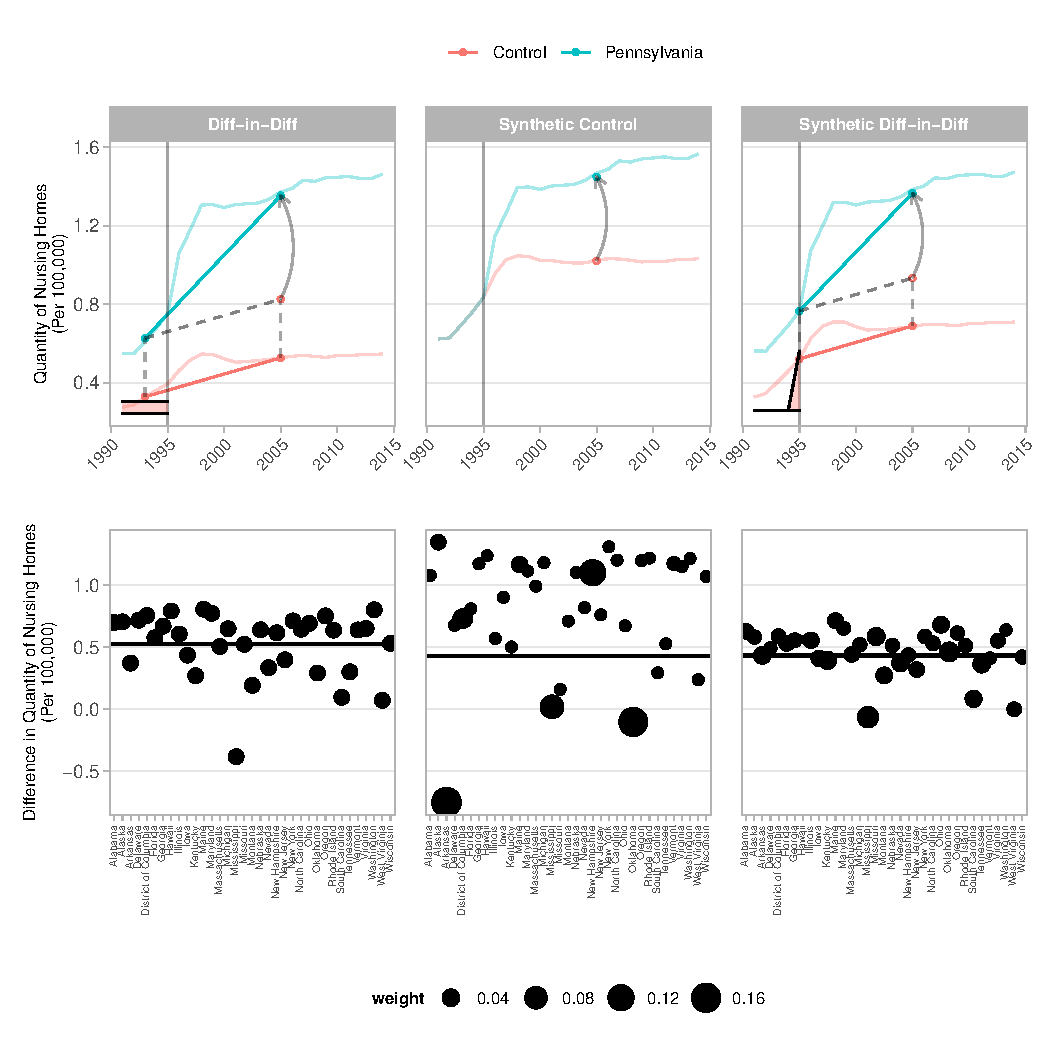
\includegraphics[width=\textwidth,keepaspectratio]{q_nursing_homes_plots_PA.pdf}
    \end{center}
    \footnotesize
		\textit{Notes}:
\end{figure}
\clearpage

\newpage
\begin{figure}[t]
	\begin{center}
	\caption{\centering Parallel Trends and Control State Contribution Plots - Quantity of Nursing Homes Per 100,000 (IN)}
    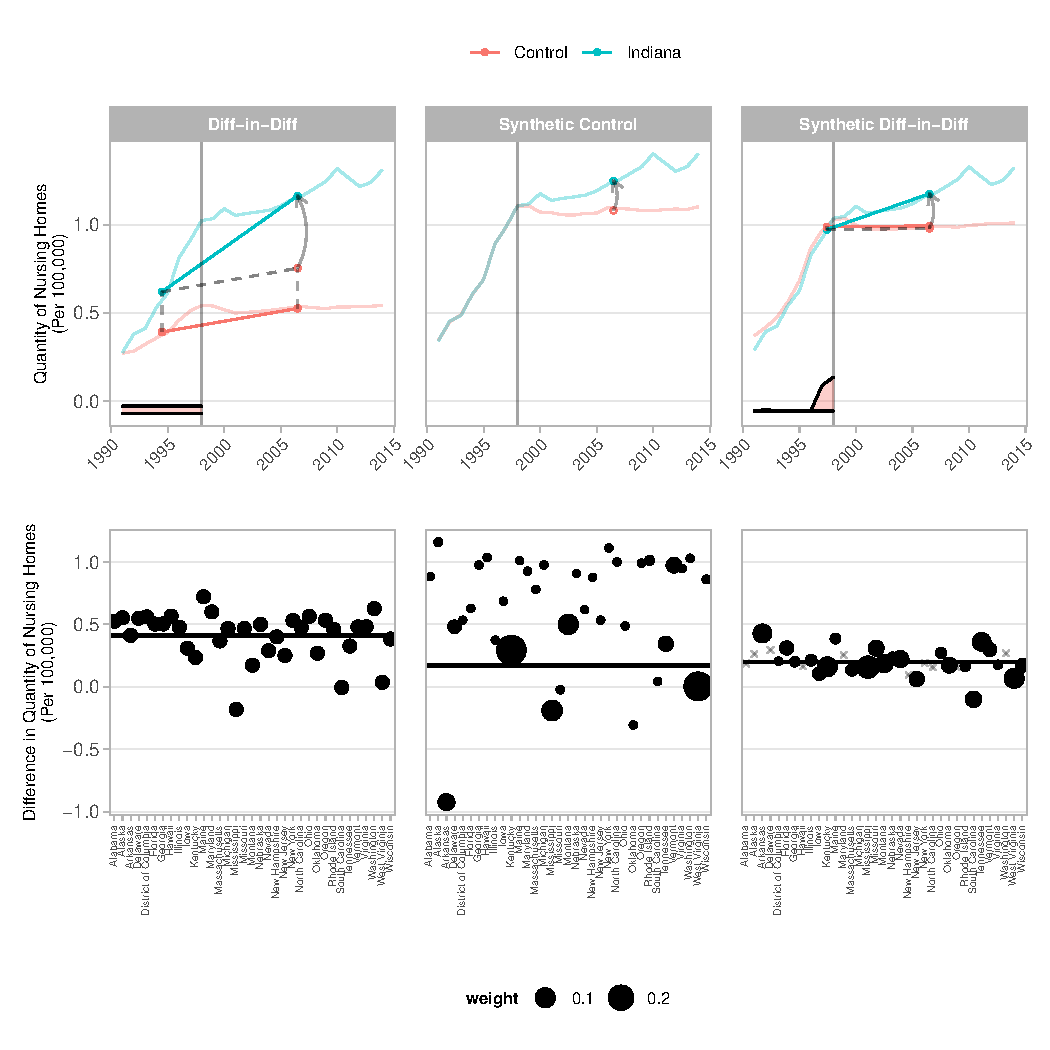
\includegraphics[width=\textwidth,keepaspectratio]{q_nursing_homes_plots_IN.pdf}
    \end{center}
    \footnotesize
		\textit{Notes}:
\end{figure}
\clearpage

\newpage
\begin{figure}[t]
	\begin{center}
	\caption{\centering Parallel Trends and Control State Contribution Plots - Quantity of Nursing Homes Per 100,000 (ND)}
    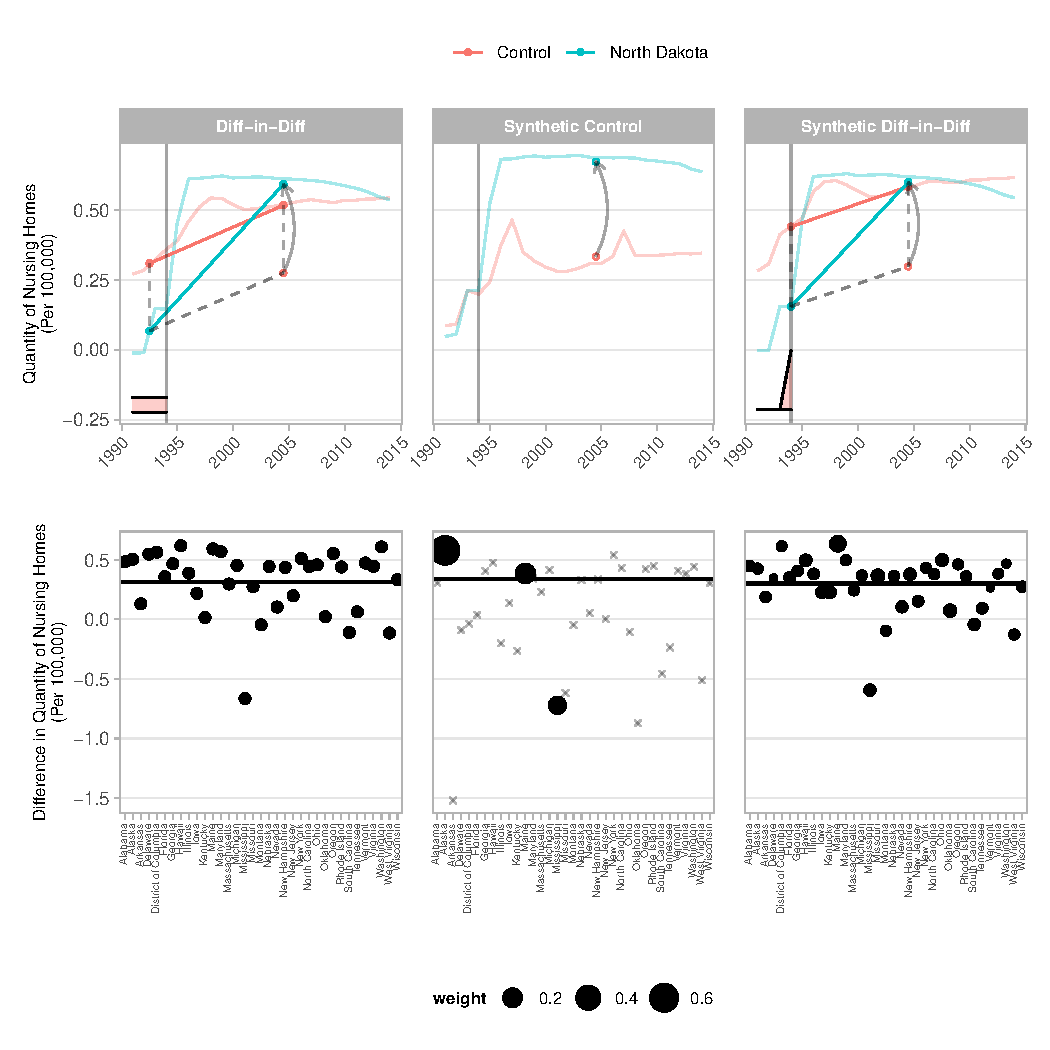
\includegraphics[width=\textwidth,keepaspectratio]{q_nursing_homes_plots_ND.pdf}
    \end{center}
    \footnotesize
		\textit{Notes}:
\end{figure}
\clearpage

\newpage
% latex table generated in R 4.1.0 by xtable 1.8-4 package
% Wed Dec 29 16:42:02 2021
\begin{table}[ht]
\centering
\begin{tabular}{lccc}
  \hline
 & Diff-in-Diff & Synthetic Control & Synthetic Diff-in-Diff \\ 
  \hline
estimate & 0.53 & 0.43 & 0.43 \\ 
  standard error & 0.24 & 0.18 & 0.16 \\ 
  95\% Confidence Interval & (0.05, 1.00) & (0.08, 0.77) & (0.12, 0.75) \\ 
   \hline
\end{tabular}
\caption{Quantity of Nursing Homes Per 100,000 - PA} 
\end{table}

% latex table generated in R 4.1.0 by xtable 1.8-4 package
% Thu Dec 30 18:28:16 2021
\begin{table}[ht]
\centering
\begin{tabular}{lccc}
  \hline
 & Diff-in-Diff & Synthetic Control & Synthetic Diff-in-Diff \\ 
  \hline
estimate & 0.41 & 0.17 & 0.2 \\ 
  standard error & 0.18 & 0.16 & 0.12 \\ 
  95\% Confidence Interval & (0.06, 0.77) & (-0.15, 0.49) & (-0.04, 0.43) \\ 
   \hline
\end{tabular}
\caption{Quantity of Nursing Homes Per 100,000 - IN} 
\end{table}

% latex table generated in R 4.1.0 by xtable 1.8-4 package
% Thu Dec 30 23:27:23 2021
\begin{table}[ht]
\centering
\begin{tabular}{lccc}
  \hline
 & Diff-in-Diff & Synthetic Control & Synthetic Diff-in-Diff \\ 
  \hline
estimate & 0.32 & 0.34 & 0.3 \\ 
  standard error & 0.26 & 0.22 & 0.21 \\ 
  95\% Confidence Interval & (-0.19, 0.82) & (-0.09, 0.77) & (-0.11, 0.71) \\ 
   \hline
\end{tabular}
\caption{Quantity of Nursing Homes Per 100,000 - ND} 
\end{table}

\clearpage






\newpage
\vspace*{8cm}
\section{Quantity of Nursing Home Beds Per 100,000}
\clearpage

\newpage
\begin{figure}[t]
	\begin{center}
	\caption{\centering Parallel Trends and Control State Contribution Plots - Quantity of Nursing Home Beds Per 100,000 (PA)}
    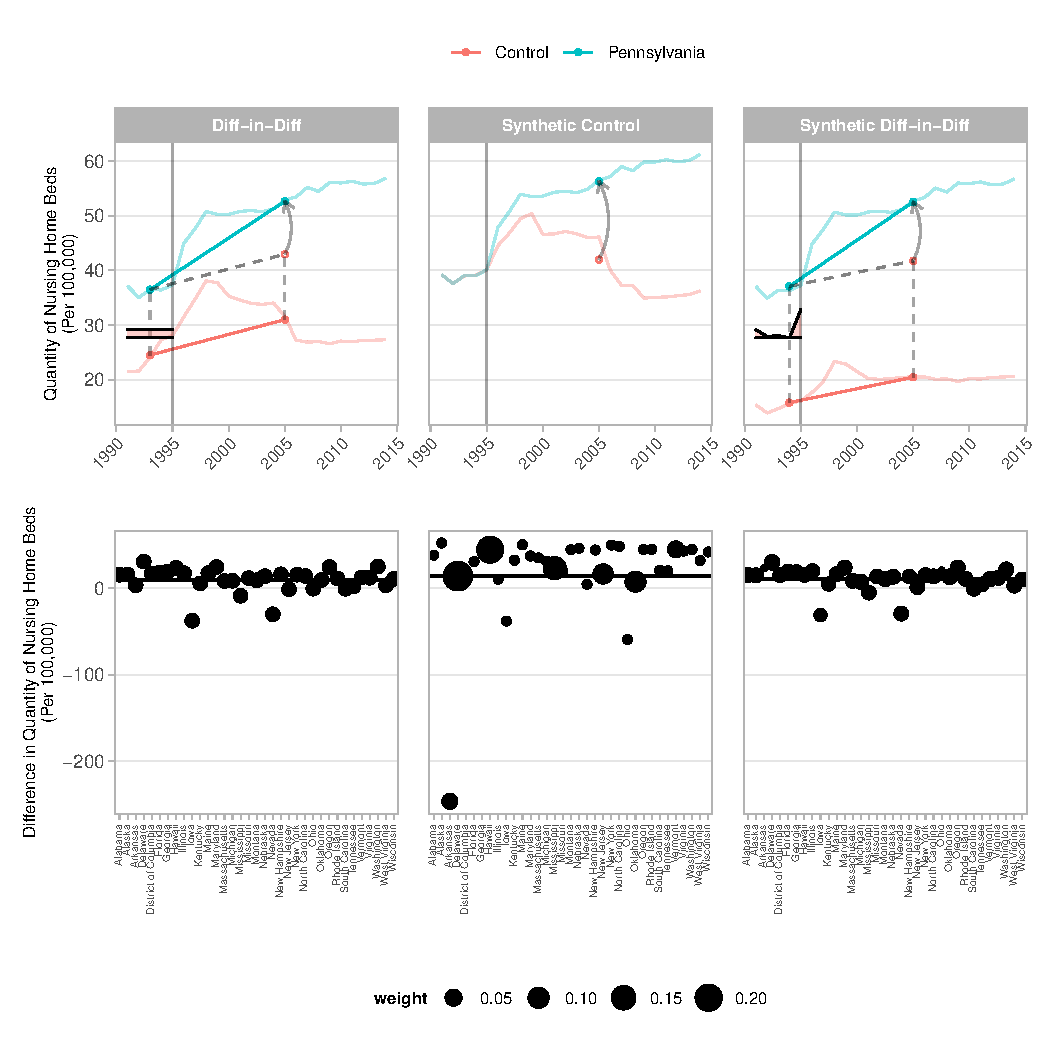
\includegraphics[width=\textwidth,keepaspectratio]{q_nursing_home_beds_plots_PA.pdf}
    \end{center}
    \footnotesize
		\textit{Notes}:
\end{figure}
\clearpage

\newpage
\begin{figure}[t]
	\begin{center}
	\caption{\centering Parallel Trends and Control State Contribution Plots - Quantity of Nursing Home Beds Per 100,000 (IN)}
    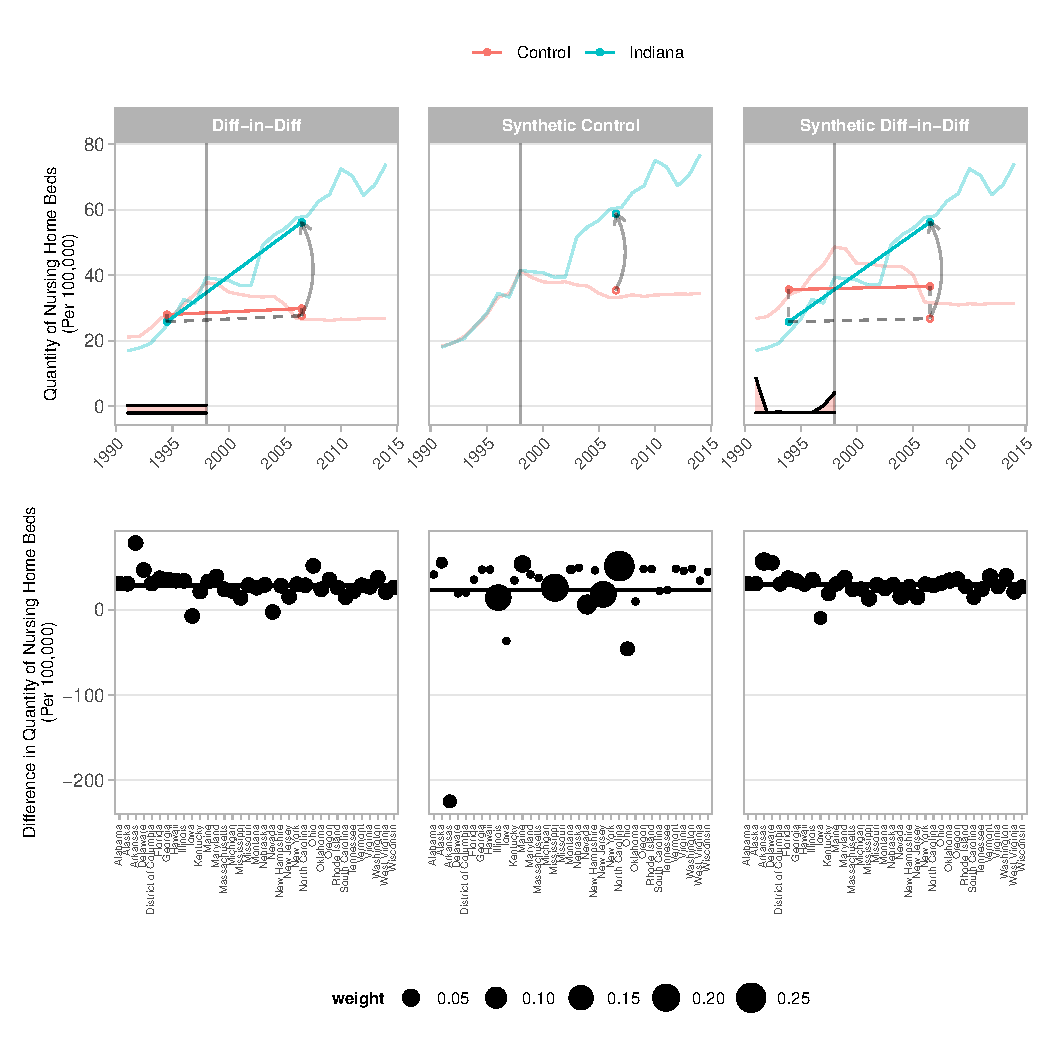
\includegraphics[width=\textwidth,keepaspectratio]{q_nursing_home_beds_plots_IN.pdf}
    \end{center}
    \footnotesize
		\textit{Notes}:
\end{figure}
\clearpage

\newpage
\begin{figure}[t]
	\begin{center}
	\caption{\centering Parallel Trends and Control State Contribution Plots - Quantity of Nursing Home Beds Per 100,000 (ND)}
    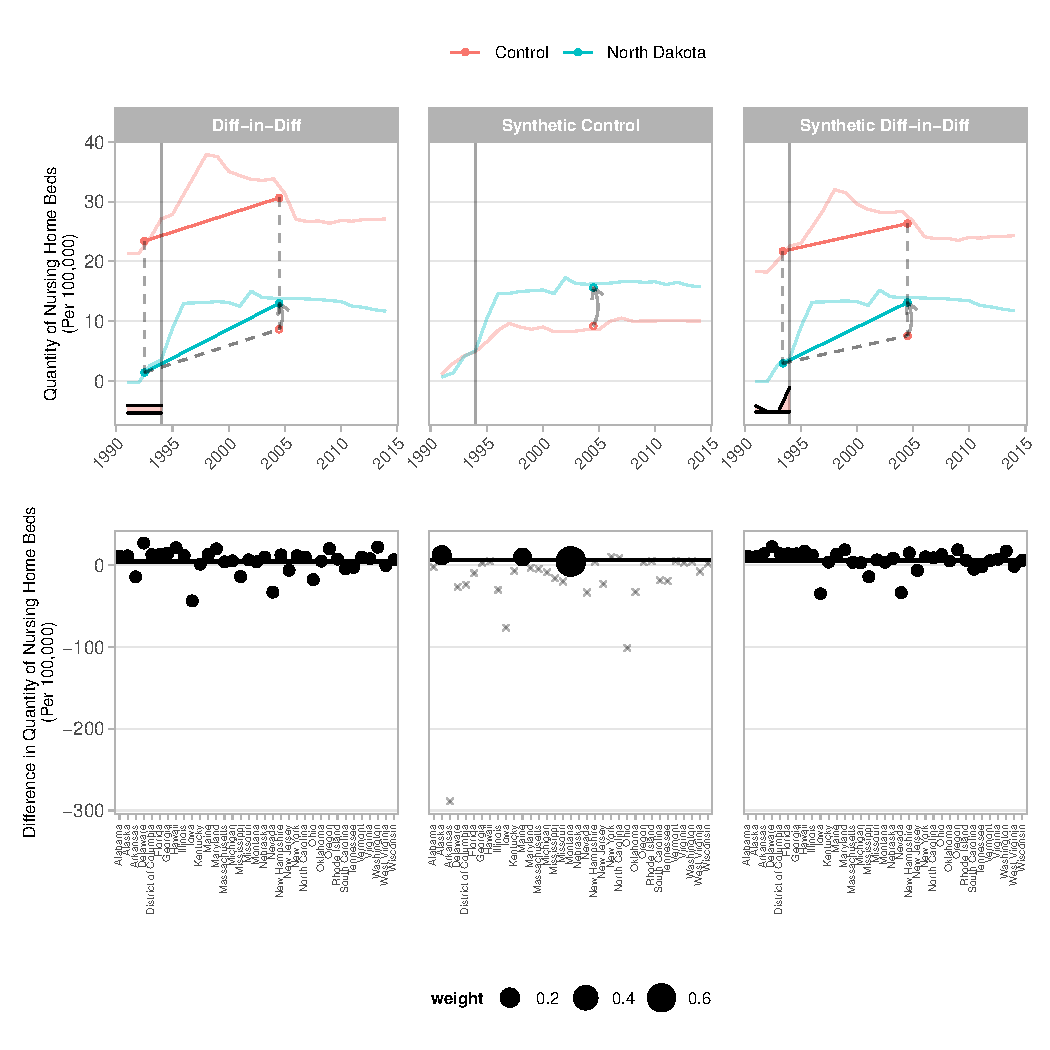
\includegraphics[width=\textwidth,keepaspectratio]{q_nursing_home_beds_plots_ND.pdf}
    \end{center}
    \footnotesize
		\textit{Notes}:
\end{figure}
\clearpage

\newpage
% latex table generated in R 4.1.0 by xtable 1.8-4 package
% Thu Dec 30 14:34:55 2021
\begin{table}[ht]
\centering
\begin{tabular}{lccc}
  \hline
 & Diff-in-Diff & Synthetic Control & Synthetic Diff-in-Diff \\ 
  \hline
estimate & 9.69 & 14.31 & 10.79 \\ 
  standard error & 13.23 & 32.15 & 12.03 \\ 
  95\% Confidence Interval & (-16.25, 35.63) & (-48.70, 77.32) & (-12.80, 34.37) \\ 
   \hline
\end{tabular}
\caption{Quantity of Nursing Home Beds Per 100,000 - PA} 
\end{table}

% latex table generated in R 4.1.0 by xtable 1.8-4 package
% Thu Dec 30 19:33:11 2021
\begin{table}[ht]
\centering
\begin{tabular}{lccc}
  \hline
 & Diff-in-Diff & Synthetic Control & Synthetic Diff-in-Diff \\ 
  \hline
estimate & 28.48 & 23.37 & 29.46 \\ 
  standard error & 13.89 & 30.25 & 13.74 \\ 
  95\% Confidence Interval & (1.27, 55.70) & (-35.93, 82.66) & (2.52, 56.39) \\ 
   \hline
\end{tabular}
\caption{Quantity of Nursing Home Beds Per 100,000 - IN} 
\end{table}

% latex table generated in R 4.1.0 by xtable 1.8-4 package
% Fri Dec 31 00:24:41 2021
\begin{table}[ht]
\centering
\begin{tabular}{lccc}
  \hline
 & Diff-in-Diff & Synthetic Control & Synthetic Diff-in-Diff \\ 
  \hline
estimate & 4.36 & 6.42 & 5.55 \\ 
  standard error & 14.73 & 32.15 & 12.22 \\ 
  95\% Confidence Interval & (-24.52, 33.23) & (-56.60, 69.44) & (-18.40, 29.50) \\ 
   \hline
\end{tabular}
\caption{Quantity of Nursing Home Beds Per 100,000 - ND} 
\end{table}

\clearpage





\newpage
\vspace*{8cm}
\section{Total Expenditure}
\clearpage

\newpage
\begin{figure}[t]
	\begin{center}
	\caption{\centering Parallel Trends and Control State Contribution Plots - Total Expenditure (PA)}
    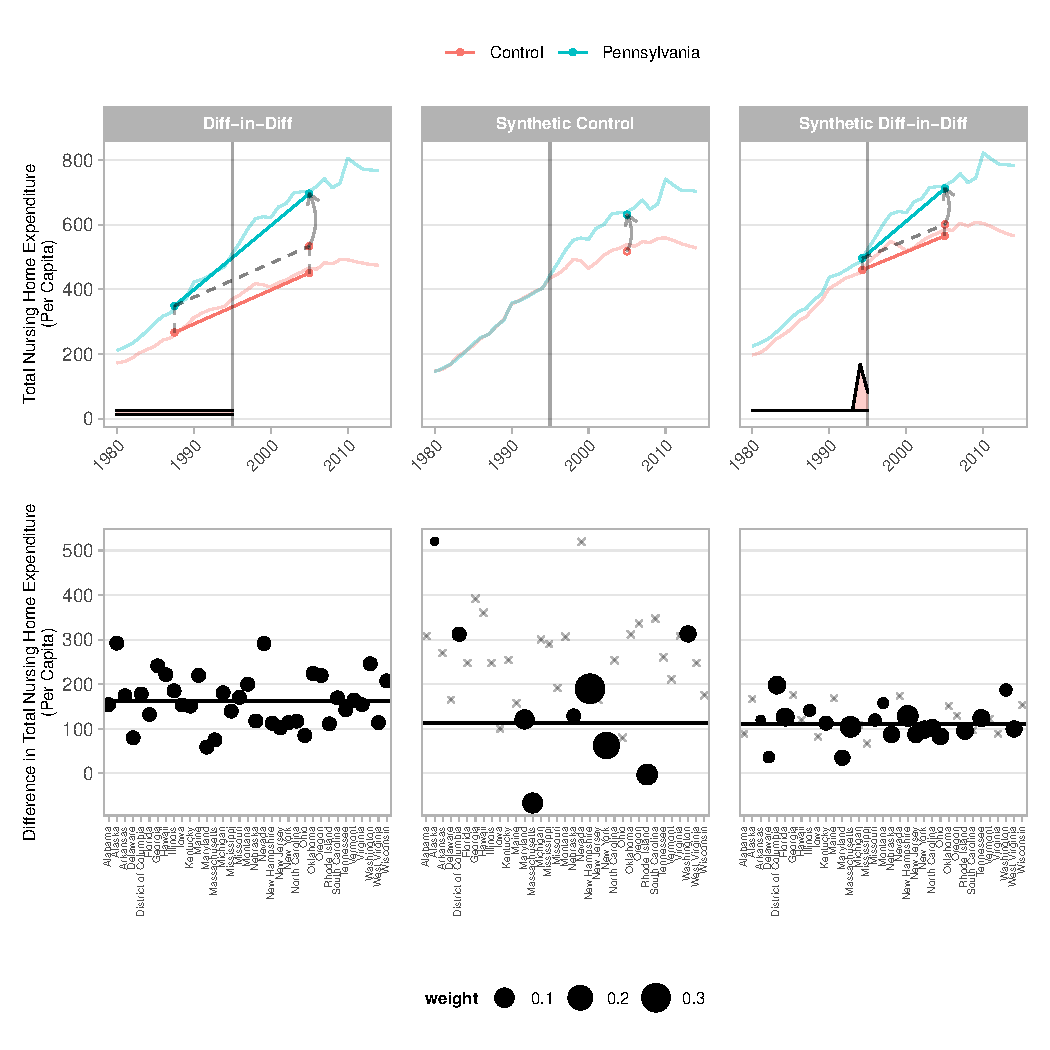
\includegraphics[width=\textwidth,keepaspectratio]{total_expenditure_plots_PA.pdf}
    \end{center}
    \footnotesize
		\textit{Notes}:
\end{figure}
\clearpage

\newpage
\begin{figure}[t]
	\begin{center}
	\caption{\centering Parallel Trends and Control State Contribution Plots - Total Expenditure (IN)}
    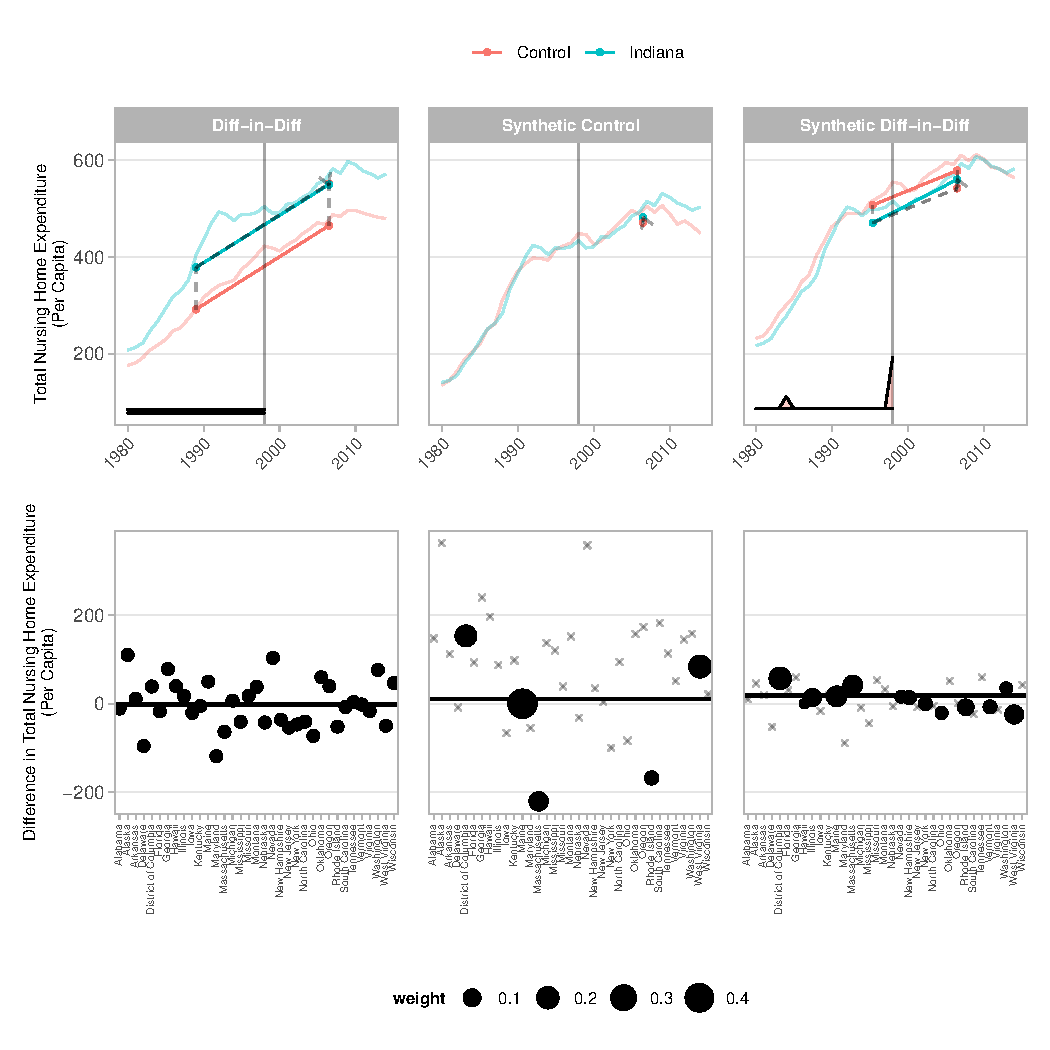
\includegraphics[width=\textwidth,keepaspectratio]{total_expenditure_plots_IN.pdf}
    \end{center}
    \footnotesize
		\textit{Notes}:
\end{figure}
\clearpage

\newpage
\begin{figure}[t]
	\begin{center}
	\caption{\centering Parallel Trends and Control State Contribution Plots - Total Expenditure (ND)}
    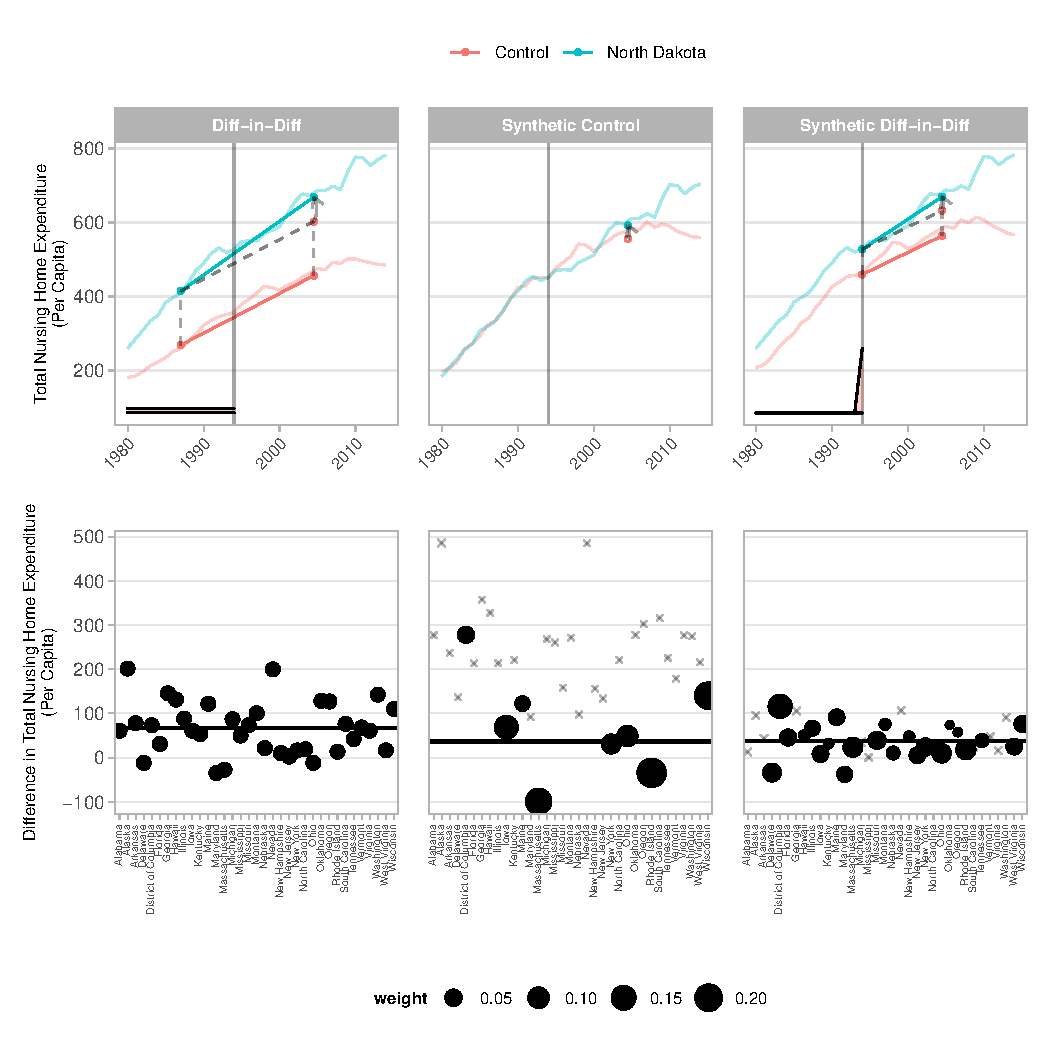
\includegraphics[width=\textwidth,keepaspectratio]{total_expenditure_plots_ND.pdf}
    \end{center}
    \footnotesize
		\textit{Notes}:
\end{figure}
\clearpage

\newpage
% latex table generated in R 4.1.0 by xtable 1.8-4 package
% Mon Dec 27 17:32:04 2021
\begin{table}[ht]
\centering
\begin{tabular}{lccc}
  \hline
 & Diff-in-Diff & Synthetic Control & Synthetic Diff-in-Diff \\ 
  \hline
estimate & 162.75 & 113.49 & 111.26 \\ 
  standard error & 53.4 & 44.89 & 44.7 \\ 
  95\% Confidence Interval & (58.09, 267.41) & (25.51, 201.47) & (23.64, 198.88) \\ 
   \hline
\end{tabular}
\caption{Total Expenditure - PA} 
\end{table}

% latex table generated in R 4.1.0 by xtable 1.8-4 package
% Thu Dec 30 21:01:20 2021
\begin{table}[ht]
\centering
\begin{tabular}{lccc}
  \hline
 & Diff-in-Diff & Synthetic Control & Synthetic Diff-in-Diff \\ 
  \hline
estimate & -1.79 & 11.04 & 18.31 \\ 
  standard error & 50.19 & 6304.24 & 34.09 \\ 
  95\% Confidence Interval & (-100.15, 96.58) & (-12345.27, 12367.35) & (-48.51, 85.13) \\ 
   \hline
\end{tabular}
\caption{Total Expenditure - IN} 
\end{table}

% latex table generated in R 4.1.0 by xtable 1.8-4 package
% Fri Dec 31 01:44:27 2021
\begin{table}[ht]
\centering
\begin{tabular}{lccc}
  \hline
 & Diff-in-Diff & Synthetic Control & Synthetic Diff-in-Diff \\ 
  \hline
estimate & 66.37 & 36.27 & 37.43 \\ 
  standard error & 53.78 & 6692.79 & 36.56 \\ 
  95\% Confidence Interval & (-39.03, 171.78) & (-13081.60, 13154.13) & (-34.23, 109.09) \\ 
   \hline
\end{tabular}
\caption{Total Expenditure - ND} 
\end{table}

\clearpage



\newpage
\vspace*{8cm}
\section{Medicaid Expenditure}
\clearpage

\newpage
\begin{figure}[t]
	\begin{center}
	\caption{\centering Parallel Trends and Control State Contribution Plots - Medicaid Expenditure (PA)}
    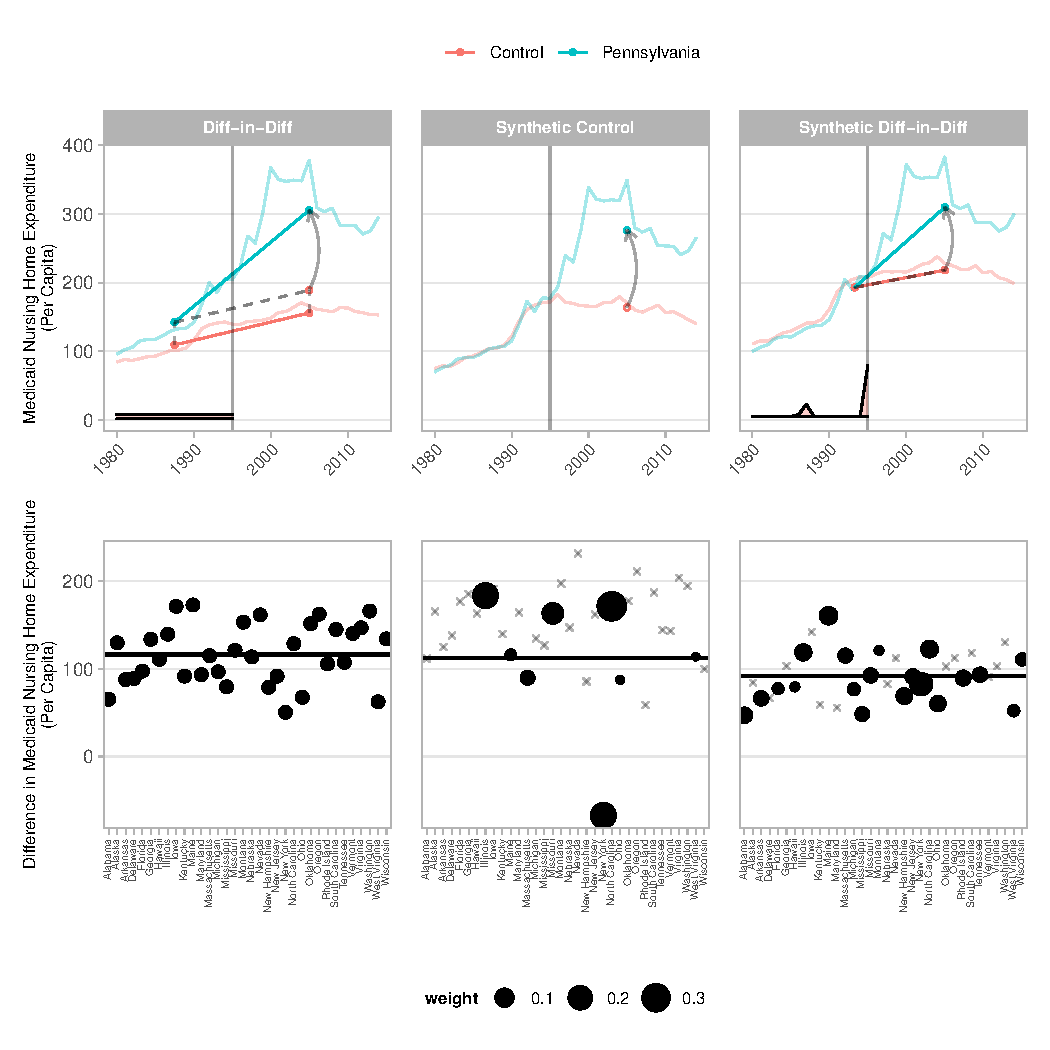
\includegraphics[width=\textwidth,keepaspectratio]{medicaid_expenditure_plots_PA.pdf}
    \end{center}
    \footnotesize
		\textit{Notes}:
\end{figure}
\clearpage

\newpage
\begin{figure}[t]
	\begin{center}
	\caption{\centering Parallel Trends and Control State Contribution Plots - Medicaid Expenditure (IN)}
    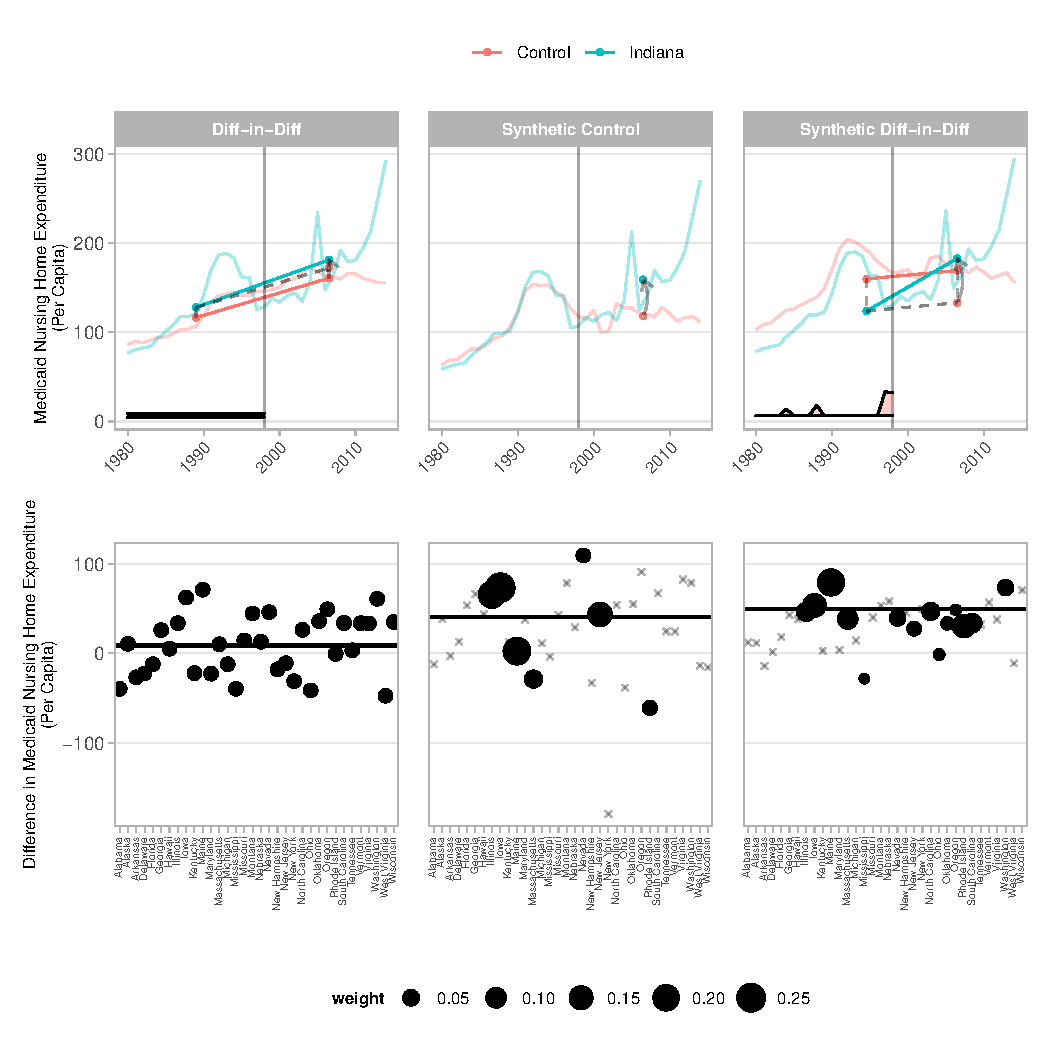
\includegraphics[width=\textwidth,keepaspectratio]{medicaid_expenditure_plots_IN.pdf}
    \end{center}
    \footnotesize
		\textit{Notes}:
\end{figure}
\clearpage

\newpage
\begin{figure}[t]
	\begin{center}
	\caption{\centering Parallel Trends and Control State Contribution Plots - Medicaid Expenditure (ND)}
    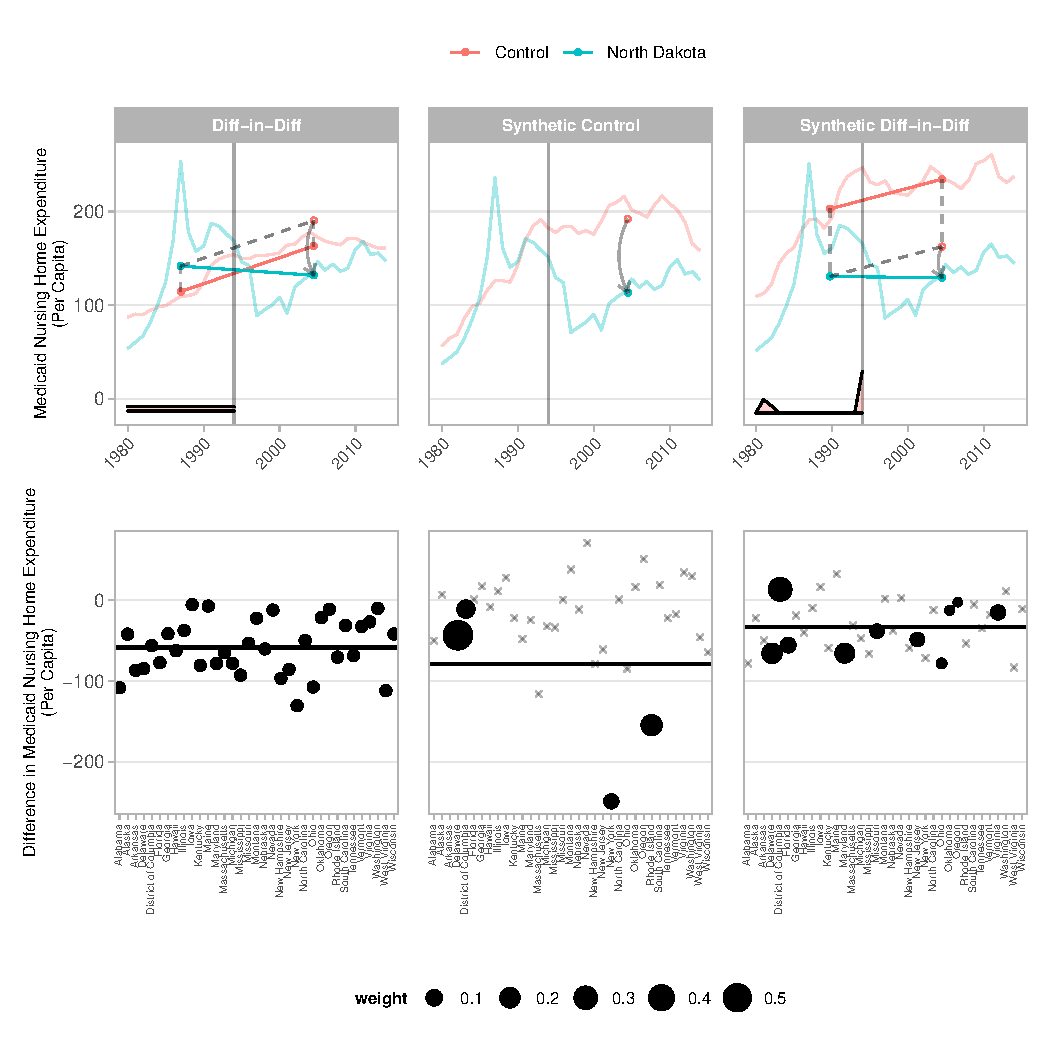
\includegraphics[width=\textwidth,keepaspectratio]{medicaid_expenditure_plots_ND.pdf}
    \end{center}
    \footnotesize
		\textit{Notes}:
\end{figure}
\clearpage

\newpage
% latex table generated in R 4.1.0 by xtable 1.8-4 package
% Wed Dec 29 14:54:27 2021
\begin{table}[ht]
\centering
\begin{tabular}{lccc}
  \hline
 & Diff-in-Diff & Synthetic Control & Synthetic Diff-in-Diff \\ 
  \hline
estimate & 117.01 & 93.19 & 98.53 \\ 
  standard error & 37.3 & 4811.04 & 31.23 \\ 
  95\% Confidence Interval & (43.90, 190.13) & (-9336.45, 9522.84) & (37.31, 159.75) \\ 
   \hline
\end{tabular}
\caption{Medicaid Expenditure - PA} 
\end{table}

% latex table generated in R 4.1.0 by xtable 1.8-4 package
% Thu Dec 30 22:30:09 2021
\begin{table}[ht]
\centering
\begin{tabular}{lccc}
  \hline
 & Diff-in-Diff & Synthetic Control & Synthetic Diff-in-Diff \\ 
  \hline
estimate & 9.99 & 60.95 & 48.52 \\ 
  standard error & 34.7 & 1094.46 & 28.03 \\ 
  95\% Confidence Interval & (-58.03, 78.00) & (-2084.19, 2206.09) & (-6.41, 103.45) \\ 
   \hline
\end{tabular}
\caption{Medicaid Expenditure - IN} 
\end{table}

% latex table generated in R 4.1.0 by xtable 1.8-4 package
% Fri Dec 31 03:04:26 2021
\begin{table}[ht]
\centering
\begin{tabular}{lccc}
  \hline
 & Diff-in-Diff & Synthetic Control & Synthetic Diff-in-Diff \\ 
  \hline
estimate & -58.5 & -78.82 & -33.26 \\ 
  standard error & 37.59 & 3535.81 & 36.28 \\ 
  95\% Confidence Interval & (-132.17, 15.16) & (-7009.01, 6851.38) & (-104.38, 37.85) \\ 
   \hline
\end{tabular}
\caption{Medicaid Expenditure - ND} 
\end{table}

\clearpage

\end{document}